\documentclass{beamer}
\usepackage{graphicx}
\usepackage{amsmath, amsthm, amsfonts, amssymb, mathrsfs}
\usepackage{textcomp} % straigth apos
\usepackage{tikz}
\usepackage{verbatim}
\usepackage{tikzit}
\usepackage{listings}
\usepackage{subfig}
\usepackage[ruled,vlined, linesnumbered]{algorithm2e}
\usepackage{algorithmic,float}


\input{graphs.tikzstyles}

% Graph notations
\def\NN{$\mathcal{N}~$}
\def\GG{$\mathcal{G}~$}
\def\VV{$\mathcal{V}~$}
\def\EE{$\mathcal{E}~$}


% Colors definition
\definecolor{isa_red}{RGB}{255, 58, 71}
\definecolor{isa_blue}{RGB}{0, 103, 158}
\definecolor{isa_green}{RGB}{0, 157, 97}
\definecolor{isa_dark_green}{RGB}{0,131, 0}
\definecolor{isa_purple}{RGB}{174, 5, 238}
\definecolor{isa_dark_blue}{RGB}{26, 0, 253}

% Isabelle keywords
\newcommand{\apply}{{\color{isa_red}{apply}}}
\newcommand{\done}{{\color{isa_red}{done}}}
\newcommand{\datatype}{{\color{isa_blue}{datatype}}}
\newcommand{\inductive}{{\color{isa_blue}{inductive}}}
\newcommand{\abbreviation}{{\color{isa_blue}{abbreviation}}}
\newcommand{\thm}{{\color{isa_blue}{theorem}}}
\newcommand{\lm}{{\color{isa_blue}{lemma}}}
\newcommand{\fun}{{\color{isa_blue}{fun}}}
\renewcommand{\locale}{{\color{isa_blue}{locale}}}
\newcommand{\where}{{\color{isa_green}{where}}}
\renewcommand{\and}{{\color{isa_green}{and}}}
\newcommand{\fixes}{{\color{isa_green}{fixes}}}
\newcommand{\assumes}{{\color{isa_green}{assumes}}}
\newcommand{\shows}{{\color{isa_green}{shows}}}
\newcommand{\generic}[1]{{\color{isa_purple}{\textquotesingle#1}}}
\newcommand{\isa}[1]{\texttt{#1}}
\newcommand{\blue}[1]{{\color{isa_dark_blue}{#1}}}
\newcommand{\green}[1]{{\color{isa_dark_green}{#1}}}

\theoremstyle{definition}
\newtheorem*{isabelle}{}

\setbeamercovered{invisible}

\setbeamertemplate{theorems}[numbered]
\setbeamertemplate{lemma}[numbered]
\newtheorem{remark}{Remark}

\usetheme{Madrid}
\useoutertheme{tree} % Alternatively: miniframes, infolines, split
\useinnertheme{circles}

\definecolor{lightbrown}{RGB}{220, 147, 91}

\usecolortheme[named=lightbrown]{structure}

\title[Présentation de mon Parcours Recherche]{Vérification formelle en Isabelle(HOL)\\d'un algorithme calculant les composantes\\ fortement connexes d'un graphe}
%% sm: not really convinced by the title -- FM in HOL sounds redundant to me
%% also are there really several algorithms?
%% maybe "Verification in HOL of an algorithm for computing SCCs" ?
\date{June 9, 2022}
\author[V. Trélat, S. Merz]{Vincent Trélat, Stephan Merz}
\institute[Mines Nancy]{\normalsize{École Nationale Supérieure des Mines de Nancy\\Département Informatique}}

\begin{document}

\begin{frame}
  \begin{figure}[t]
    \centering
    
\includegraphics[height=30pt]{img/logoartem.png}
    \hspace{1cm}
    
\includegraphics[height=32pt]{img/logoloria.jpg}
    \hspace{1cm}
    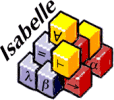
\includegraphics[height=32pt]{img/logoisabelle.png}
  \end{figure}
  \titlepage
\end{frame}

\section{Présentation et intérêt des méthodes formelles}
\begin{frame}
  \tableofcontents
\end{frame}

\subsection{Programmation défensive}
\begin{frame}
    \onslide<1->{
        \begin{center}
            Comment garantir le fonctionnement continu d'un logiciel dans des conditions imprévues ?
        \end{center}
        \vfill
    }
    \begin{itemize}
        \item<2-> Concepts de Sofwtare Engineering (design documents, design patterns, etc.)
        \item<2-> Review de code en équipe (GitHub, etc.)
        \item<2-> Séries de tests (unitaires, d'intégration, fonctionnels, etc.)
    \end{itemize}
    \vfill
    \onslide<3->{
        $\Longrightarrow$ Responsabilité du programmeur !
    }
\end{frame}

\begin{frame}
    \onslide<1->{
        \begin{quotation}
            Probability of human error is considerably higher than that of machine error.
            \begin{flushright}
                Kenneth Appel
        \end{flushright}
        % Kenneth Appel est un mathématicien qui a démontré le théorème des 4 couleurs (problème 4-COL) en 1976 :
        % Il est possible, en n'utilisant que 4 couleurs, de colorier n'importe quelle carte découpée en régions connexes, de sortes que deux régions adjacentes soient toujours de couleur différente.
    \end{quotation}
    }
    \onslide<2->{
        \begin{figure}
            \centering
            \subfloat{
                
\includegraphics[height=3.5cm]{img/4col.png}
            }
            \subfloat{
                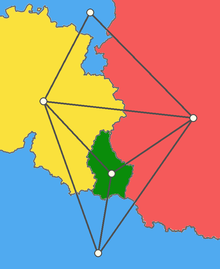
\includegraphics[height=3.5cm]{img/4col2.png}
            }
        \caption{Illustrations du problème 4-COL}
        \end{figure}
    % Première preuve assistée par ordinateur ! Explosion combinatoire dûe au nombre de cas à explorer. Débat à l'époque sur la validité de la preuve.
    }
\end{frame}

\subsection{Les méthodes formelles}
\begin{frame}
    En méthodes formelles, on considère un programme comme une structure mathématique, ce qui permet de raisonner dessus de manière formelle.
    % les méthodes formelles sont des techniques permettant de raisonner rigoureusement, à l'aide de logique mathématique, sur un programme informatique, afin de démontrer sa validité par rapport à une certaine spécification. Elles reposent sur les sémantiques des programmes, c'est-à-dire sur des descriptions mathématiques formelles du sens d'un programme donné par son code.
    \vfill
    \begin{itemize}
        \item Rigueur
        \item Concepts de logique
        \item Sémantique
        \item Validité par rapport à des spécifications
    \end{itemize}
\end{frame}

\begin{frame}
    \begin{center}
        Preuve papier vs. preuve formelle
    \end{center}
    \begin{itemize}
        \item L'utilisateur fournit la structure de la preuve
        \item Automatisation des preuves
        \item Différents outils informatiques : assistants à la preuve (Isabelle(HOL), Coq, Why3, B, etc.) et model checkers (TLC, etc.)
    \end{itemize}
\end{frame}

\section{Vérification formelle en Isabelle}
\begin{frame}
    ...
\end{frame}

\end{document}